\documentclass{beamer}

%% Fonts and encodings
\usepackage{multicol}
\usepackage{mathabx}
\usepackage[scaled]{helvet}
\usepackage{color}
\usepackage{lmodern}
\usepackage{eulervm}
\usepackage{wasysym}
\usefonttheme[onlymath]{serif}
\usefonttheme{professionalfonts}
\usefonttheme{structurebold}
\hypersetup{backref}
\usepackage{bm}
\usepackage[utf8x]{inputenc}
\usepackage{booktabs}
%% Color & Theme
\definecolor{SUblue}{RGB}{0,0,180}
\usecolortheme[RGB={0,0,180}]{structure}
\usetheme{Boadilla}
\setbeamertemplate{navigation symbols}{}
\setbeamertemplate{itemize items}[circle]
\setbeamertemplate{enumerate items}[circle]

\setbeamerfont{title}{size=\large}
\setbeamerfont{frametitle}{size=\normalsize}
\setbeamerfont{framesubtitle}{size=\small, shape =$\color{violet}{\looparrowdownright}~$}
\setbeamercolor{title}{fg=white, bg= SUblue!75!green}
\setbeamercolor{framesubtitle}{fg=violet}

\title[Covariate-contingent copulas]{{\textbf{Modeling covariate-contingent
      correlation and tail dependence with copulas}}}



\author[Feng Li]{\includegraphics[height=2cm]{cufelogo}\\
\vspace{0.5cm}\textbf{Feng Li}}
\institute[Stat \& Math, CUFE]{\footnotesize{\textbf{School of Statistics and
      Mathematics\\ Central University of Finance and Economics}}}
\date{}

\begin{document}

% \begin{frame}[plain]
% \includegraphics[width=\textwidth]{FERM2014AD}
% \end{frame}


%% Title page
\begin{frame}[plain]
  \addtocounter{framenumber}{-1}
  \titlepage
\end{frame}

%% Outline
\section*{Outline of the talk}
\begin{frame}
  \frametitle{Outline of the talk}
  \addtocounter{framenumber}{-1}
  \tableofcontents
\end{frame}

%%%%%%%%%%%%%%%%%%%%%%%%%%%%%%%%%%%%%%%%%%%%%%%%%%%%%%%%%%%%%%%%%%%%%%%%%%%%%%%%
%% The main slides
%%%%%%%%%%%%%%%%%%%%%%%%%%%%%%%%%%%%%%%%%%%%%%%%%%%%%%%%%%%%%%%%%%%%%%%%%%%%%%%%

\section{A financial story}
 \begin{frame}
  \frametitle{The stock market returns}
    \begin{figure}
      \centering
      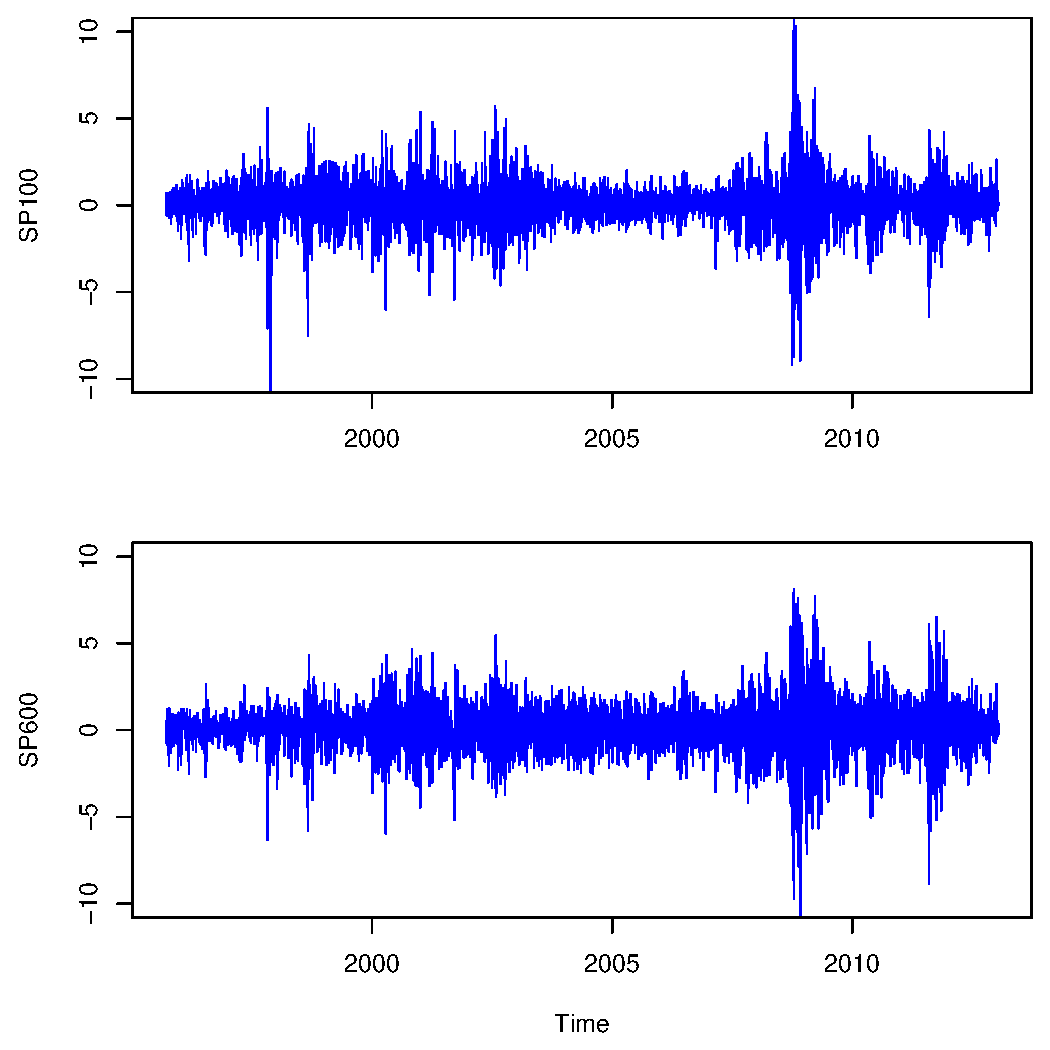
\includegraphics[height=0.9\textheight]{SP100-SP600}
    \end{figure}
\end{frame}

\begin{frame}
  \frametitle{Our interests}
  \begin{itemize}

  \item We would like to construct a multivariate model that some margins are
    continuous but some are discrete.

    \begin{itemize}
    \item One margin: A company's stock credited as $A$, $A^+$ over time by
      Standard \& Poor's.
    \item The other margin: the stock returns over time
    \end{itemize}

  \item In the \emph{big data} world: we would like to estimate a very heavy multivariate
    model in such way that
    \begin{enumerate}
    \item Independently build each marginal model. Parallel them!
    \item Build the multivariate dependences on top of the margins.
    \end{enumerate}

  \end{itemize}
\end{frame}


%\section{Introduction to copulas}
\begin{frame}
  \frametitle{Introduction to copulas}
  \framesubtitle{What is a copula?}
  \begin{itemize}
  \item The word ``copula'' means \textbf{linking}.
  \item \textbf{Sklar's theorem}

    Let $H$ be a multi-dimensional distribution function with marginal
    distribution functions $F_1(x_1),...,F_m(x_m)$. Then there exists a
    function $C$ (\textbf{copula function}) such that
    \begin{equation*}
      \begin{split}
        H(x_1,...,x_m)= & C(F_1(x_1),...,F_m(x_m))\\
        =&C\left(\int_{-\infty}^{x_1}f(z_1)dz_1,...,\int_{-\infty}^{x_m}f(z_m)dz_m\right)=C(u_1,...,u_m).
      \end{split}
    \end{equation*}
    Furthermore, if $F_i(x_i)$ are continuous, then $C$ is unique, and the derivative $c(u_1,...,u_m)= \partial^m C(u_1,...,u_m)/(\partial u_1...
    \partial u_m)$ is the \textbf{copula density}.

  \end{itemize}
\end{frame}

\begin{frame}
  \frametitle{Introduction to copulas}
  \framesubtitle{Some arbitrary examples}
  \begin{itemize}

  \item If $X_1,...,X_m$ are independent, and iff $C$ is a product copula, then
    \begin{equation*}
      C(F_1(x_1),...,F_m(x_m))=\prod \nolimits _{i=1}^{m} F_i(x_i)
    \end{equation*}

  \item The bivariate Gaussian copula
    \begin{equation*}
      \begin{split}
        &C(u_1,u_2,\rho)=\Phi_2(\Phi^{-1}(u_1),\Phi^{-1}(u_2),\rho)\\
        &= \int_{-\infty}^{\Phi^{-1}(u_1)}\int_{-\infty}^{\Phi^{-1}(u_2)}
        \frac{1}{2\pi\sqrt{1-\rho^2}}\exp\left\{- \frac{z_1^2-2\rho z_1z_2+z_2^2}{2(1-\rho^2)} \right\}\mathrm{d}z_1\mathrm{d}z_2
      \end{split}
    \end{equation*}

  \item The multivariate probit model is a simple example of a Gaussian copula,
    with univariate probit regressions as the marginals.

  \item  There are many ways to construct a copula youself.
  \end{itemize}
\end{frame}

\section{Measuring correlation and tail dependence with copulas}
\begin{frame}
  \frametitle{Measuring correlation and tail dependence}
  \framesubtitle{Kendall's $\tau$ and tail-dependences}
  \begin{itemize}
  \item The \textbf{Kendall's $\tau$} can be written in terms of copula function:
    \begin{equation*}
      \begin{split}
        \tau = & 4 \int \int F(x_1, x_2)dF(x_1,x_2)-1 = 4 \int \int C(u_1, u_2)dC(u_1,u_2)-1. \\
      \end{split}
    \end{equation*}

  \item As well as the bivariate lower and upper \textbf{tail dependences}
    \begin{equation*}
      \begin{split}
        \lambda_L = & \lim \limits_{u \to 0^{+}} Pr(X_1< F_1^{-1}(u)| X_2<F_2^{-1}(u))= \lim \limits_{u \to 0^{+}} \frac{C(u,u)}{u},\\
        \lambda_U=&\lim \limits_{u \to 1^{-}} Pr(X_1> F_1^{-1}(u)|
        X_2>F_2^{-1}(u))= \lim \limits_{u \to 1^{-}} \frac{1-C(u,u)}{1-u}.\\
      \end{split}
    \end{equation*}

  \item Some facts:
    \begin{itemize}
    \item The Kendall's $\tau$ is invariant w.r.t. \textbf{strictly} increasing transformations.
    \item For all copulas in the elliptical class (Gaussian, \emph{t},...),
      $\tau = \frac{2}{\pi}arcsin(\rho)$.
    \item The Gaussian copula has zero tail dependence.
    \item The  student \texttt{t} copula has asmptotic upper tail dependence even for negative
      and zero correlations. The tail dependence decreases when degrees of
      freedom increases.
    \end{itemize}
  \end{itemize}
\end{frame}

\section{The covariate-contingent copula model}
\begin{frame}
  \frametitle{The covariate-contingent copula model}
  \framesubtitle{The Joe-Clayton copula}
  \begin{itemize}
  \item The Joe-Clayton copula function
    \[
    \begin{split}
      C(u,v,\theta,\delta)=&1-\left[1-\left\{\left(1-\bar u ^{\theta }\right)^{-\delta
          }+\left(1-\bar v ^{\theta }\right)^{-\delta }-1\right\}^{-1/\delta
        }\right]^{1/\theta }
    \end{split}
    \]
    where $\theta \geq 1$, $\delta > 0$, $\bar u = 1-u$, $\bar v = 1-v$ .

  \item Some properties:
    \begin{itemize}
    \item One type of Archimedean copula.
    \item $\lambda_L=2^{-1/\delta}$ does not depend on $\lambda_U=2-2^{-1/\theta}$.
    \item  $\tau=1- 4\int _0^{\infty} s\times(\varphi'(s))^2ds$ is calculated via Laplace transform.
    \end{itemize}

  \item Our interests:
    \begin{itemize}
    \item The rank correlation and tail dependence in the model.
    \item The convenience for interpretation (knowing the underlying factors of
      dependences).
    \end{itemize}

  \item We use the reparameterized copula    $C(u,v,\lambda_L,
    \tau)=C(u,v,\theta,\delta)$.
  \item [*] \textbf{Note!} any other copulas can be equally well used.
  \end{itemize}

\end{frame}

\begin{frame}[plain]
  % \frametitle{The covariate-contingent copula model}
  % \framesubtitle{The dependence and correlation of Joe-Clayton copula}
  \begin{figure}
    \centering
    \vspace{-0.35cm}
    \includegraphics[width=0.46\textwidth]{BB7_tau-lamba.pdf}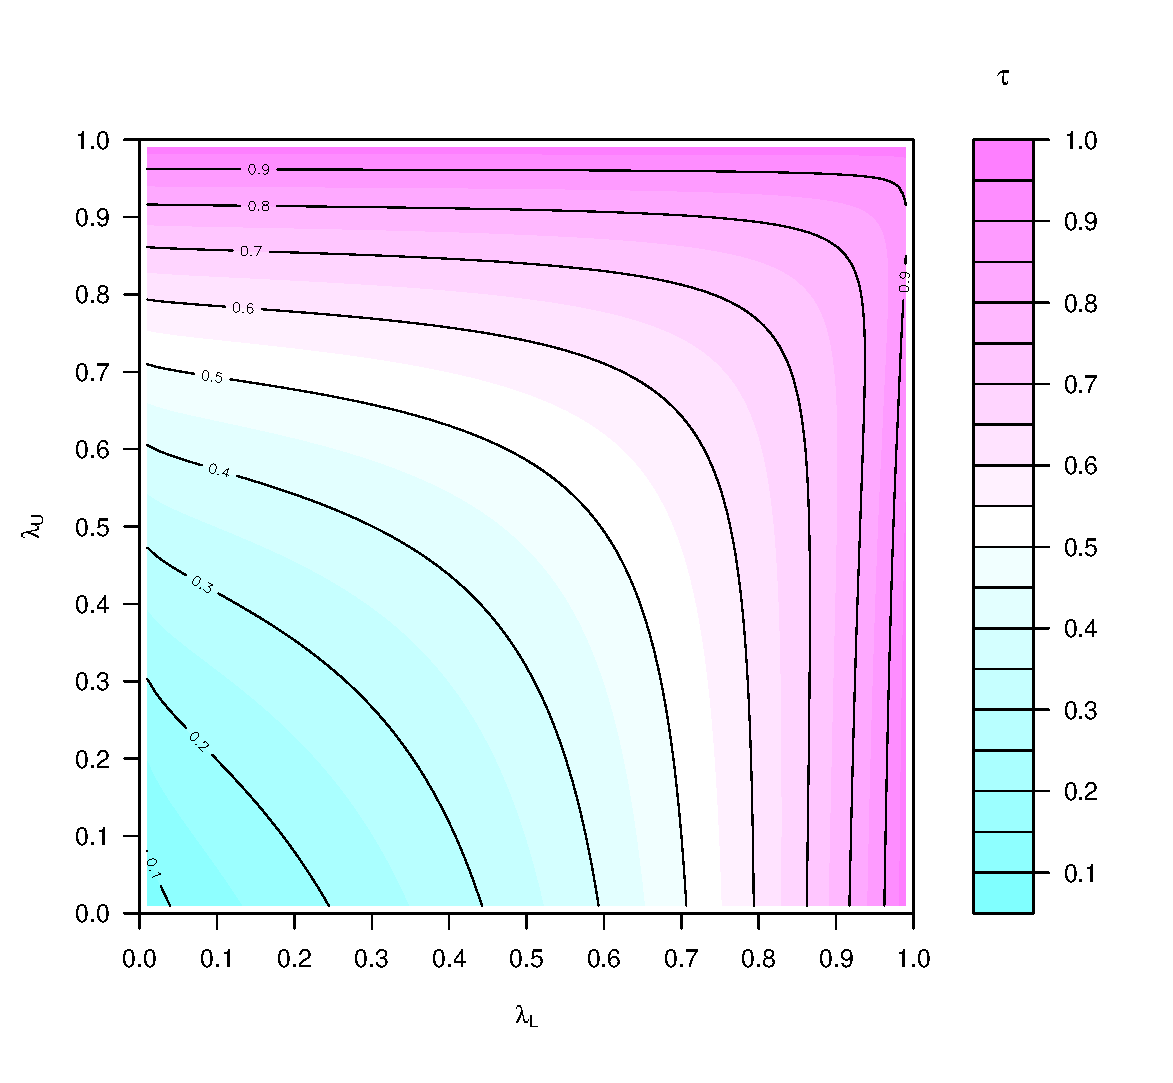
\includegraphics[width=0.56\textwidth]{tau-contour}\\
    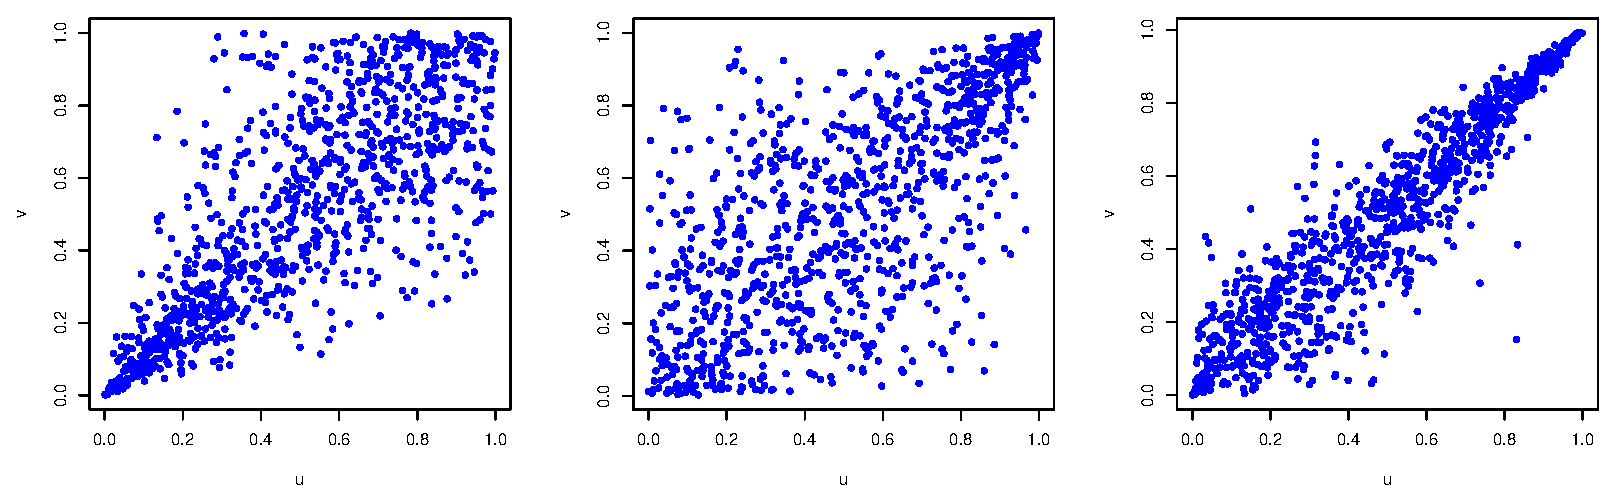
\includegraphics[width=\textwidth]{BB7Scatter.eps}
  \end{figure}
\end{frame}

\begin{frame}
  \frametitle{The covariate-contingent copula model}
  \framesubtitle{The model}
  \begin{itemize}
  \item \textbf{The marginal models}
    \begin{itemize}
    \item In principle, any combination of univariate marginal models can be
      used.
    \item In the continuous case, we use univariate model that each margin is
      from the student \emph{t} distribution.
    \end{itemize}
  \item \textbf{The log likelihood}
\[
\begin{split}\log p(\{\bm{\beta},\bm{\mathcal{I}}\}|\bm{y},\bm{x})= & \mathrm{constant}+\sum\nolimits _{j=1}^{M}\log p(\bm{y}_{.j}|\{\bm{\beta},\bm{\mathcal{I}}\}_{j},\bm{x}_{j})\\
 & +\log\mathcal{L}_{C}(\bm{u}|\{\bm{\beta},\bm{\mathcal{I}}\}_{C},\bm{y},\bm{x})+\log p(\{\bm{\beta},\bm{\mathcal{I}}\})
\end{split}
\]

    % \begin{equation*}
    %   \begin{split}
    %     & \log \mathcal{L} (Y_u,Y_v| X_u, X_v,\lambda_L, \tau,\beta_u,\beta_v) =  \sum_{i=1}^{n}
    %     \log c(u_i,v_i, \lambda_L, \tau) \\
    %     & \hspace{2.8cm}  + \log \mathcal{L}_u(Y_u|X_u,\beta_u) + \log \mathcal{L}_v(Y_v|X_v,\beta_v)\\
    %   \end{split}
    % \end{equation*}
    where all the parameters are connected with covariates via link function
    $\varphi(\cdot)$, (identity, log, logit, probit,...)
    \begin{center}
      \begin{tabular}{lll}
        Marginal features&$\mu = \varphi_{\beta_u}^{-1}(X_u\beta_u),$
        &$\sigma^2 = \varphi_{\beta_\sigma}^{-1}(X_\sigma\beta_\sigma),$ ... \\
        Copula features&$\lambda_L = \varphi_{\lambda}^{-1}((X_u,X_v)\beta_\lambda),$& $\tau = \varphi_{\tau}^{-1}((X_u,X_v)\beta_\tau).$ \\
      \end{tabular}
    \end{center}
  \end{itemize}
\end{frame}

% \begin{frame}
%   \frametitle{The covariate-contingent copula model}
%   \framesubtitle{The fast approach}

%   \begin{itemize}
%   \item Estimate each marginal model.
%   \item Conditional on each marginal model, estimate the copula features
%   \end{itemize}


% \end{frame}


\begin{frame}
  \frametitle{The covariate-contingent copula model}
  \framesubtitle{The Bayesian approach}
  \begin{itemize}

  \item The priors

    \begin{itemize}

    \item The priors for the copula functions are easy to specify due to our
      reparameterization.

    \item  The priors for the marginal distributions are specified in their usual
      ways.

    \item When variable selection is used, we assume there are no covariates in
      the link functions \emph{a priori}.

    \end{itemize}

  \item The posterior
    \begin{equation*}
      p(\bm{\beta}|\bm{Y})~ \propto~ \mathcal{L} (\mathbf{Y}| \beta) \times
      \prod \limits_{i \in u,v,\tau,\lambda} p(\beta_i)
    \end{equation*}

  \item The posterior inference is straightforward although the model is very complicated.
  \end{itemize}
\end{frame}

\begin{frame}
  \frametitle{The covariate-contingent copula model}
  \framesubtitle{Sampling the posterior with an efficient MCMC method}
  \begin{itemize}
  \item We update all the parameters jointly by using
    Metropolis-Hastings within Gibbs.
  \item The proposal density for each parameter vector $\beta$ is a multivariate \emph{t}-density with  $df>2$,
    \[
    \bm{\beta}_{p} |\bm{\beta}_{c}\sim\bm{MVT}\left[\bm{\hat{\beta}},~\left.-\left(\frac{\partial^{2}\ln
            p(\bm{\beta}|\bm{Y})}{\partial\bm{\beta}\partial\bm{\beta}^{\prime}}\right)^{-1}\right\vert
      _{\bm{\beta}=\bm{\hat{\beta}}},~df\right],
    \]
    where $\bm{\hat{\beta}}$ is obtained by $R$ steps ($R\leq 3$) Newton's
    iterations during the proposal with analytical gradients.

  \item Variable selections are carried out simultaneously.

  \item \textbf{The key:} The analytical gradients require the derivative for
    the copula density and marginal densities.

  % \item It is eventually straightforward. Thanks to the chain rule!

  \end{itemize}
\end{frame}

% \begin{frame}
%   \frametitle{We did everything in R}
%   \begin{itemize}
%   \item Build a fast version of R
%     \begin{itemize}
%     \item Compile R from source (with Intel \texttt{icc}, \texttt{ifort}) and
%       link it with optimized BLAS (OpenBLAS or Intel MKL) and LAPACK.
%     \item Compile the R scripts.
%    \end{itemize}

%     \item Vectorized the code whenever possible.
%     \item Parallel computing for cross-validation.


%   \end{itemize}
% \end{frame}

\begin{frame}[plain]
  \addtocounter{framenumber}{-1}

  \begin{center}
    {\Large \color{blue}{\textbf{The stock returns, a revisit}}}
  \end{center}
\end{frame}

% \begin{frame}
% %  \frametitle{The stock returns, a revisit}
%   \begin{table}
% %\caption{Description of variables in the S\&P100 and S\&P600 data.}


% \label{tab:sp-covariates}

% \centering %
% \begin{tabular}{lp{0.7\textwidth}l}
% \toprule
% Variable & Description & \tabularnewline
% \midrule
% \textsf{Return}  & Daily return $y_{t}=100\log(p_{t}/p_{t-1})$ where $p_{t}$ is the
% closing price. & \tabularnewline
%  &  & \tabularnewline
% \textsf{RM1/5/20} & Return of last day/week/month. & \tabularnewline
% \textsf{CloseAbs95} & Geometrically decaying average of absolute returns $(1-\rho)\sum\nolimits _{s=0}^{\infty}\rho^{s}|y_{t-2-s}|$
% with $\rho=0.95$. & \tabularnewline
% \textsf{CloseAbs80} & Geometrically decaying average of past absolute returns with $\rho=0.80$. & \tabularnewline
% \textsf{MaxMin95} & Measure of volatility $(1-\rho)\sum\nolimits _{s=0}^{\infty}\rho^{s}(\log(p_{t-1-s}^{h})-\log(p_{t-1-s}^{l}))$
% with $\rho=0.95$, where $p^{h}$ and $p^{l}$ are the highest and
% lowest prices. & \tabularnewline
% \textsf{MaxMin80} & Measure of volatility with $\rho=0.80$. & \tabularnewline
% \textsf{CloseSqr95} & Geometrically decaying average of returns $((1-\rho)\sum\nolimits _{s=0}^{\infty}\rho^{s}y_{t-2-s}^{2})^{1/2}$
% with $\rho=0.95$. & \tabularnewline
% \textsf{CloseSqr80} & Geometrically decaying average of returns with $\rho=0.80$. & \tabularnewline
% \bottomrule
% \end{tabular}
% \end{table}

% \end{frame}


\begin{frame}
  \begin{figure}
    \centering
    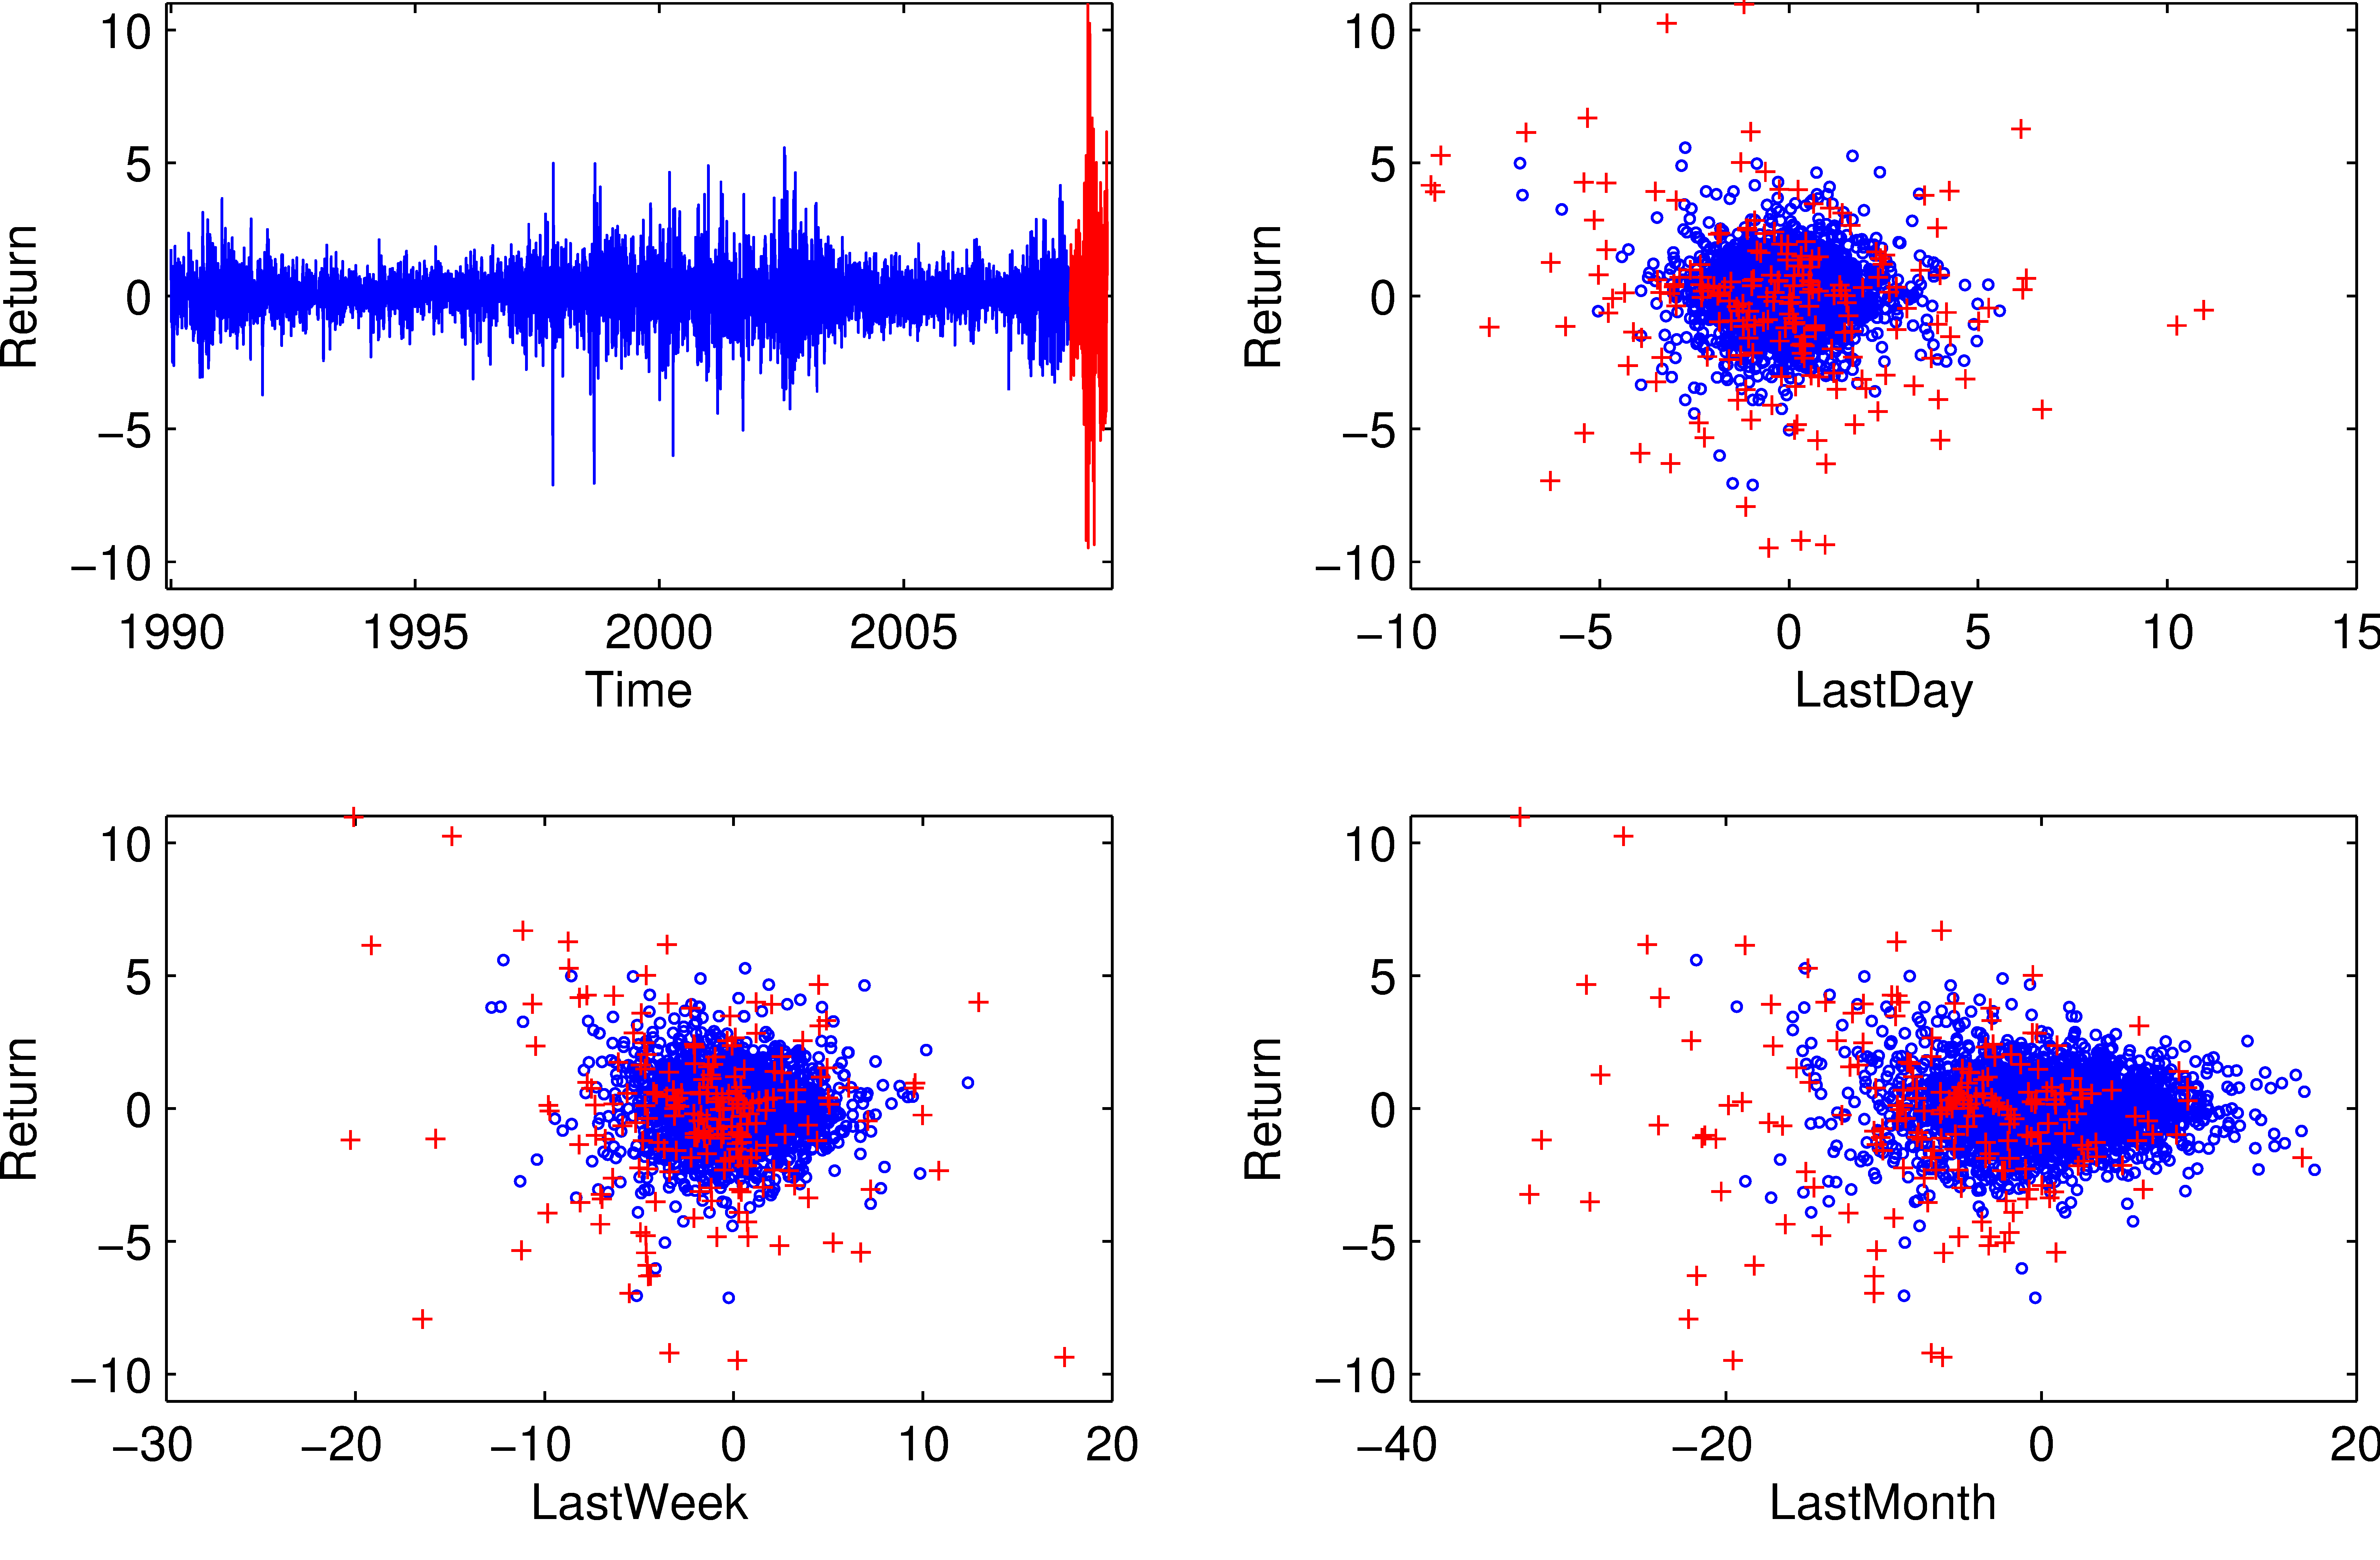
\includegraphics[height=0.8\textheight]{SP500}
  \end{figure}
\end{frame}


\begin{frame}
  \frametitle{The tail-dependence and Kendall's $\tau$ over time}
  \begin{figure}
    \centering
    
\includegraphics[height=0.34\textheight]{var-post}\\
    
\includegraphics[height=0.35\textheight]{tau-post}
  \end{figure}
\end{frame}


\begin{frame}
  \frametitle{The posterior copula plot}
  \begin{figure}
    \centering
    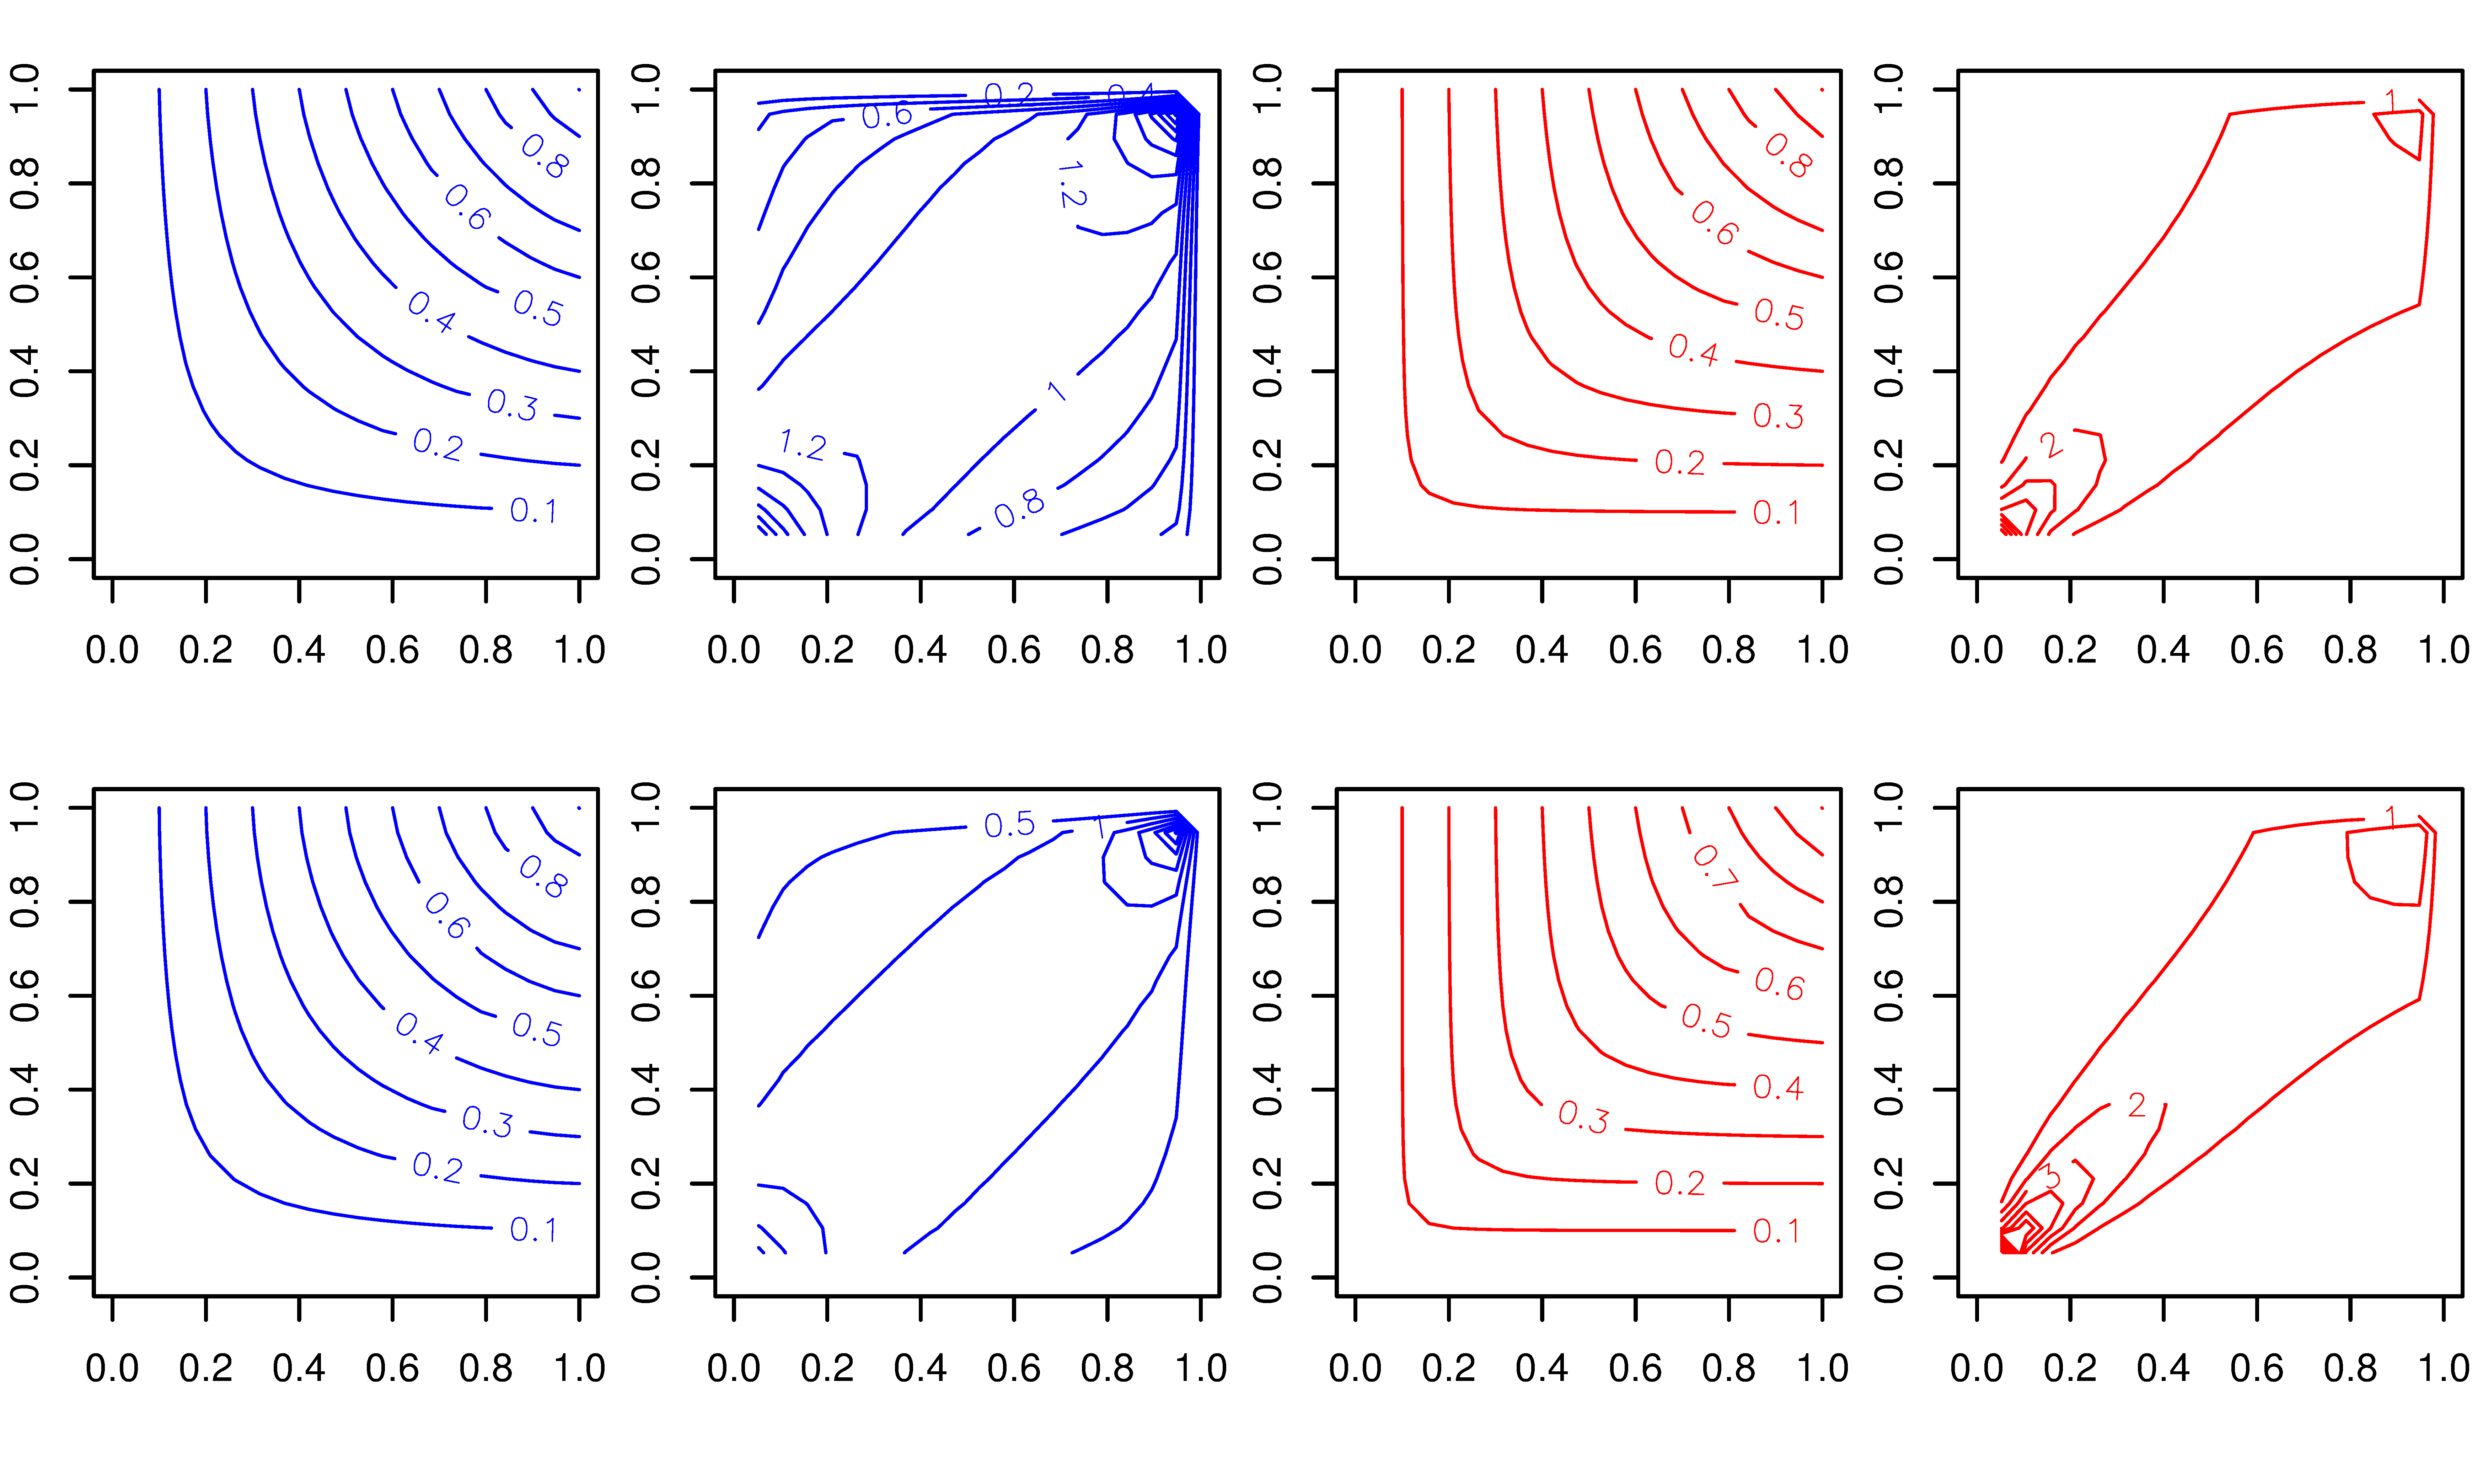
\includegraphics[height=0.8\textheight]{contour}
  \end{figure}
\end{frame}


\begin{frame}
\begin{table}
  \caption{Posterior summary of copula model with S\&P100 and S\&P600 data. In
    the copula component part, the first row and second row for $\beta$ and $\mathcal{I}$ are the results for the
    combined covariates that are used in the first and second marginal model,
    respectively. The intercept are always included in the model.}
  \label{tab:sp-fullrun}
  \centering
  \resizebox{\columnwidth}{!}{%
    \begin{tabular}{rrrrrrrrrrr}
    \toprule
    &\textsf{Intercept}&\textsf{RM1}&\textsf{RM5}&\textsf{RM20}
    &\textsf{CloseAbs95}& \textsf{CloseAbs80}& \textsf{MaxMin95}
    & \textsf{MaxMin80}&\textsf{CloseSqr95}& \textsf{CloseSqr80}\\

    \cmidrule(r){2-11}
\vspace{0.1cm}\\
\multicolumn{11}{c}{Copula component ($C$)}\\
\vspace{0.05cm}\\

$\beta_{\lambda_L}$&$-8.165$&$\mathbf{-0.555}$&$1.793$&$\mathbf{0.005}$&$-0.170$&$\mathbf{0.110}$&$-0.667$&$-1.448$&$-0.636$&$0.050$\\
               &&$\mathbf{1.463}$&$\mathbf{0.405}$&$0.934$&$-2.138$&$-1.288$&$-1.954$&$-1.577$&$\mathbf{-1.873}$&$-1.805$\\
\\
$\mathcal{I}_{\lambda_L}$&$1.00$&$\mathbf{0.98}$&$0.37$&$\mathbf{0.63}$&$0.02$&$\mathbf{0.61}$&$0.36$&$0.35$&$0.39$&$0.29$\\
                    &&$\mathbf{1.00}$& $\mathbf{1.00}$&$0.00$&$0.30$&$0.35$&$0.40$&$0.00$&$\mathbf{0.61}$&$0.34$\\

&\\

$\beta_{\tau}$&$-1.726$&$0.181$&$-0.217$&$-0.304$&$-0.107$&$\mathbf{0.115}$&$\mathbf{0.005}$&$\mathbf{-0.257}$&$\mathbf{1.068}$&$0.037$\\
             && $\mathbf{-0.191}$&$\mathbf{0.170}$&$0.274$&$0.144$&$\mathbf{-0.051}$&$\mathbf{-0.671}$&$0.059$&$-0.209$&$-0.181$\\
\\
$\mathcal{I}_{\tau}$& $1.00$&$0.00$&$0.00$&$0.00$&$0.00$&$\mathbf{0.90}$&$\mathbf{0.99}$&$\mathbf{1.00}$&$\mathbf{0.85}$&$0.00$\\
                  & &$\mathbf{1.00}$&$\mathbf{1.00}$&$0.00$&$0.00$&$\mathbf{1.00}$&$\mathbf{1.00}$&$0.00$&$0.00$&$0.00$\\


\bottomrule
  \end{tabular}
}
\flushleft \footnotesize{The inefficiency factors for the parameters are all bellow $25$.}
\end{table}
\end{frame}

\section{Extensions}
\begin{frame}
  \frametitle{Extensions and future work}
  \begin{itemize}
  \item Our bivariate tail-dependence method can be other higher-order multivariate models.
  \item Mixtures of copulas.
  \item Modeling multivariate volatility surface with copulas
  \item Our copula method is general and can also be applied to other areas,
    e.g. optimal design for multivariate data.

  \end{itemize}
\end{frame}



\begin{frame}[plain]
  \addtocounter{framenumber}{-1}
  \begin{center}
    {\color{SUblue} \textbf{\Huge Thank you!}}
    \vspace{1cm}

    {\texttt{\textbf{\url{feng.li@cufe.edu.cn}}}}

    \vspace{1cm}

    {\texttt{\textbf{\url{http://feng.li/}}}}

  \end{center}
\end{frame}

\end{document}
